\documentclass[a4paper, 11pt]{article}
\usepackage{amsmath}
\usepackage{graphicx}
\usepackage{geometry}
\usepackage{listings}
\usepackage{makecell}
\usepackage{multirow}
\geometry{scale=0.8}
\linespread{1.5}
\usepackage{hyperref}

\title{	
\normalfont \normalsize
\textsc{School of Data and Computer Science, Sun Yat-sen University} \\ [25pt] %textsc small capital letters
\rule{\textwidth}{0.5pt} \\[0.4cm] % Thin top horizontal rule
\huge  P02  CSP and KRR\\ % The assignment title
\rule{\textwidth}{2pt} \\[0.5cm] % Thick bottom horizontal rule
\author{Suixin Ou \and Yangkai Lin}
\date{September 28, 2020}
}

\begin{document}
\maketitle
\tableofcontents
\newpage







\section{Futoshiki (GAC, C++/Python)}
\subsection{Description}
Futoshiki is a board-based puzzle game, also known under the name Unequal. It is playable on a square board having a given fixed size ($4\times4$ for example), please see Figure \ref{fig:futoshiki}.

The purpose of the game is to discover the digits hidden inside the board's cells; each cell is filled with a digit between 1 and the board's size. On each row and column each digit appears exactly once; therefore, when revealed, the digits of the board form a so-called Latin square.

At the beginning of the game some digits might be revealed. The board might also contain some inequalities between the board cells; these inequalities must be respected and can be used as clues in order to discover the remaining hidden digits.

Each puzzle is guaranteed to have a solution and only one.

You can play this game online: \url{http://www.futoshiki.org/}.
\begin{figure}[h]
  \centering
  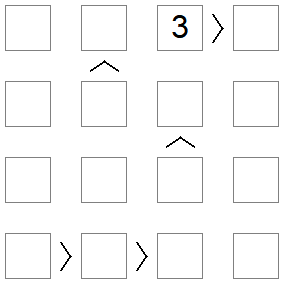
\includegraphics[width=6cm]{Pic/futoshiki1}
  \qquad
  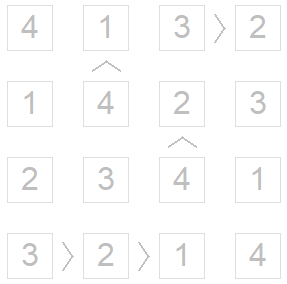
\includegraphics[width=6cm]{Pic/futoshiki2}
  \caption{Futoshiki Puzzles}
  \label{fig:futoshiki}
\end{figure}

\subsection{Tasks}

\begin{enumerate}
\item Describe with sentences the main ideas of the GAC algorithm and the main differences between the GAC and the forward checking (FC) algorithm. (10 points)
\item %When enforcing GAC on constraint $C$, if for a variable $V$ in the scope of $C$, we remove a value $d$ from CurDom[V], why do we need to check again for the consistency of any constraint containing $V$ in its scope? Some student suggests that we do not need to check again for the consistency of $C$. Is this correct, and why?

     The GAC$\_$Enforce procedure from class acts as follows: when removing d from CurDom[V], push all constraints $C'$ such that $V\in scope(C')$ and $C'\not\in$ GACQueue onto GACQueue. What's the reason behind this operation? Can it be improved and how? (20 points)

\item Use the GAC algorithm to implement a Futoshiki solver by \textbf{C++} or \textbf{Python}. (20 points)
\item Explain any ideas you use to speed up the implementation. (10 points)
\item Run the following 5 test cases to verify your solver's \textbf{correctness}. We also provide test file ``datai.txt" for every test case i. Refer to the ``readme.txt" for more details. (20 points)
\item Run the FC algorithm you implemented in E04 and the GAC algorithm you implemented in Task 3 on the 5 test cases, and fill in the following table. In the table,
    ``Total Time" means the total time the algorithm uses to solve the test case,  ``Number of Nodes Searched" means the total number of nodes traversed by the algorithm, 
    and ``Average Inference Time Per Node" means the average time for constraint propagation (inference) 
used in each node (note that this time is not equal to the total time divided by the number of nodes searched). Analyse the reasons behind the experimental results, and write them in your report. (20 points)
\setlength{\tabcolsep}{2mm}{

\begin{tabular}{|p{1.5cm}<{\centering}|p{2.2cm}<{\centering}|p{3cm}<{\centering}|p{3.3cm}<{\centering}|p{3.3cm}<{\centering}|}
\hline
Test Case&Algorithm&Total Time& Number of Nodes Searched&Average Inference Time Per Node\\
\hline
\multirow{2}*{1}&FC & & & \\
\cline{2-5}&GAC & & & \\
\hline
\multirow{2}*{2}&FC & & & \\
\cline{2-5}&GAC & & & \\
\hline
\multirow{2}*{3}&FC & & & \\
\cline{2-5}&GAC & & & \\
\hline
\multirow{2}*{4}&FC & & & \\
\cline{2-5}&GAC & & & \\
\hline
\multirow{2}*{5}&FC & & & \\
\cline{2-5}&GAC & & & \\
\hline
\end{tabular}}
\\

    \begin{figure}[htbp]
    \centering
    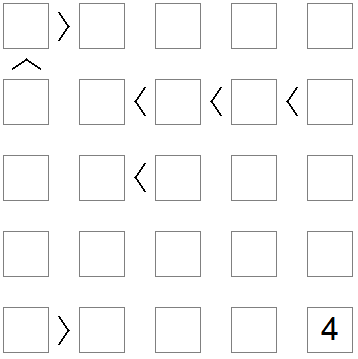
\includegraphics[width=5cm]{Pic/f1}
    \qquad
    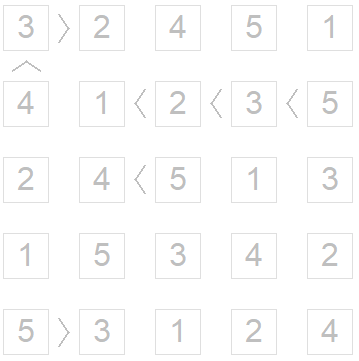
\includegraphics[width=5cm]{Pic/f1s}
    \caption{Futoshiki Test Case 1}
    \label{fig:case11}
  \end{figure}
        \begin{figure}[htbp]
    \centering
    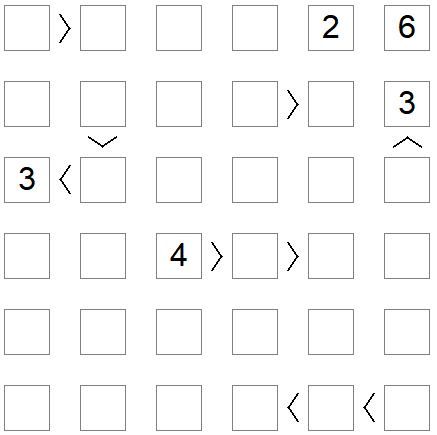
\includegraphics[width=5.5cm]{Pic/f2}
    \qquad
    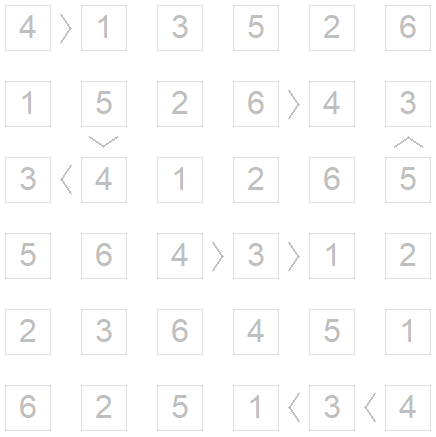
\includegraphics[width=5.5cm]{Pic/f2s}
    \caption{Futoshiki Test Case 2}
    \label{fig:case22}
  \end{figure}
        \begin{figure}[htbp]
    \centering
    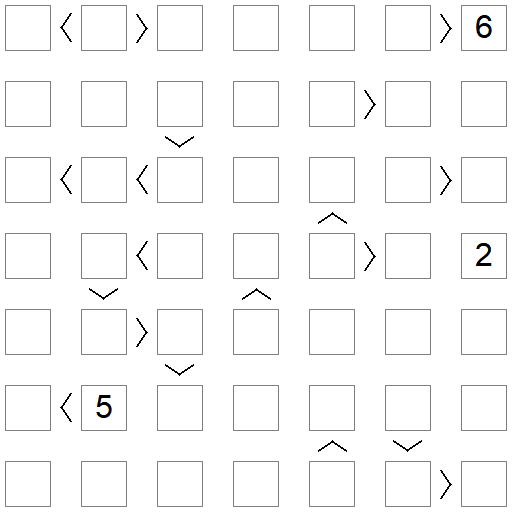
\includegraphics[width=6cm]{Pic/f3}
    \qquad
    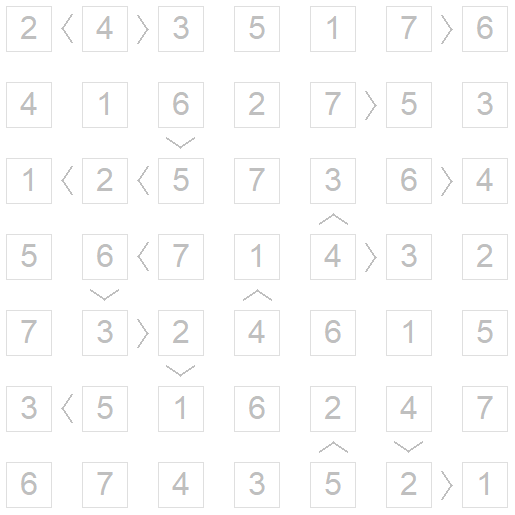
\includegraphics[width=6cm]{Pic/f3s}
    \caption{Futoshiki Test Case 3}
    \label{fig:case33}
  \end{figure}
        \begin{figure}[htbp]
    \centering
    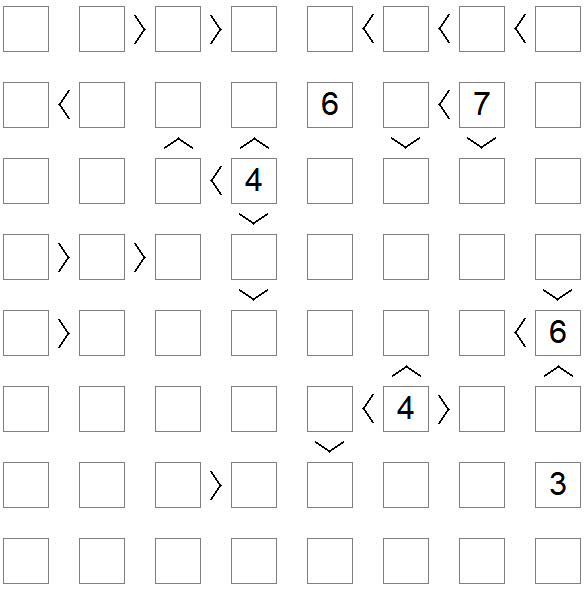
\includegraphics[width=6.5cm]{Pic/f4}
    \qquad
    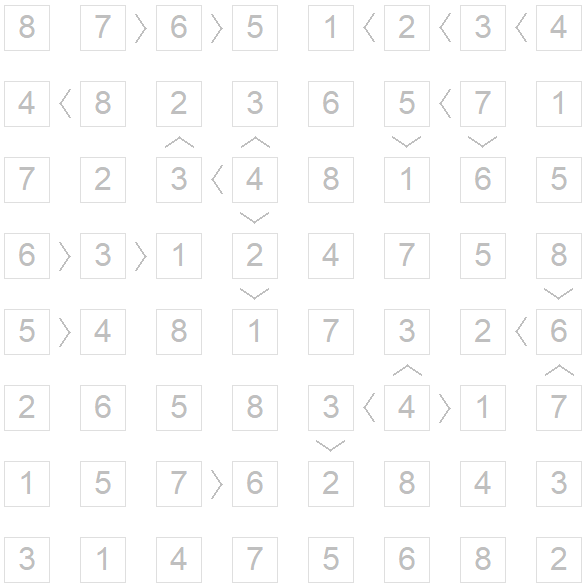
\includegraphics[width=6.5cm]{Pic/f4s}
    \caption{Futoshiki Test Case 4}
    \label{fig:case44}
  \end{figure}
        \begin{figure}[htbp]
    \centering
    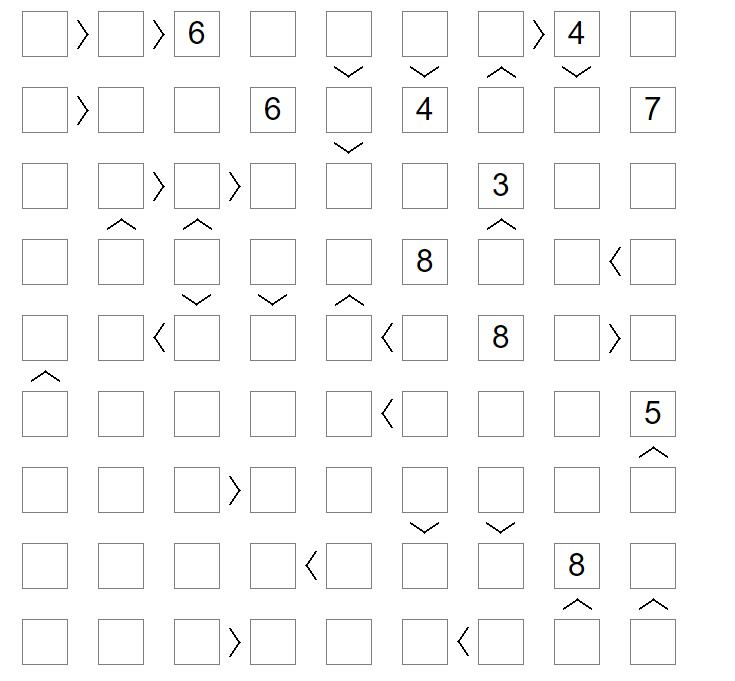
\includegraphics[width=7.5cm]{Pic/f5}
    \qquad
    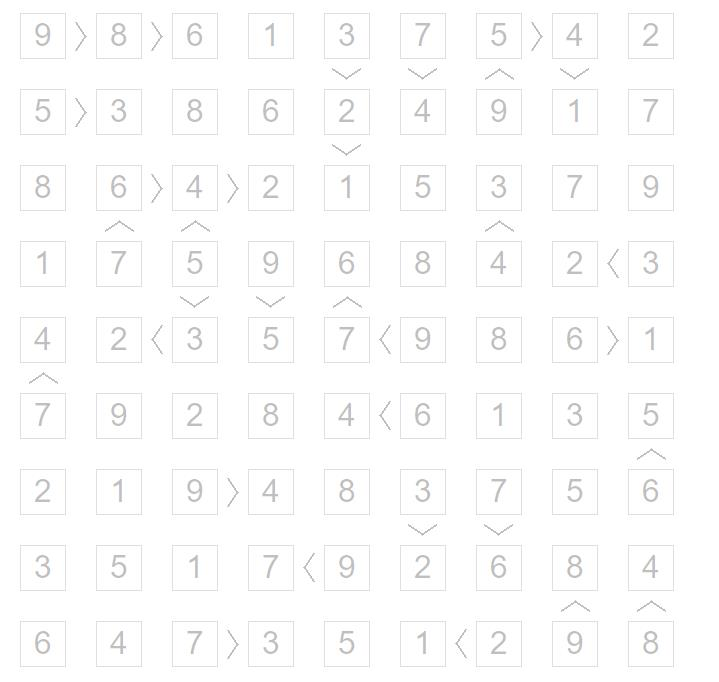
\includegraphics[width=7.5cm]{Pic/f5s}
    \caption{Futoshiki Test Case 5}
    \label{fig:case55}
  \end{figure}

\end{enumerate}


\section{Resolution}

\begin{enumerate}
\item  Implement the MGU algorithm. (10 points)
\item Using the MGU algorithm, implement a system to decide via resolution if a set of first-order clauses is satisfiable.
The input of your system is a file containing a set of first-order clauses.
In case of unsatisfiability, the output of your system is a derivation of the empty clause where each line is in the form of ``R[8a,12c]clause". Only include those clauses that are useful in the derivation. (10 points)
\item Explain any ideas you use to improve the search efficiency. (5 points)

\item Run your system on the examples of hardworker(sue), 3-blocks, Alpine Club. Include your input and output files in your report. (15 points)

\item What do you think are the main problems for using resolution to check for satisfiability for a set of first-order clauses? Explain. (10 points)

\end{enumerate}
\end{document}



%\clearpage
%\bibliography{E:/Papers/LiuLab}
%\bibliographystyle{apalike}
\end{document}
%%% Local Variables:
%%% mode: latex
%%% TeX-master: t
%%% End:
